\section{Fairness in machine learning}

\only<article>{
  The problem of fairness in machine learning and artificial intelligence has only recently been widely recognised. When any algorithm is implemented at scale, no matter the original objective and whether it is satisfied, it has significant societal effects. In particular, even when considering the narrow objective of the algorithm, even if it improves it overall, it may increase inequality.

  In this course we will look at two aspects of fairness. The first has to do with disadvantaged populations that form distinct social classes due to a shared income stratum, race or gender. The second has to do with meritocratic notions of fairness.
}
\begin{frame}
  \frametitle{Bail decisions}
  \only<article>{
    For our example regarding disadvantaged populations, consider the example of bail decisions in the US court system. When a defendant is charged, the judge has the option to either place them in jail pending trial, or set them free, under the condition that the defendant pays some amount of bail. The amount of bail (if any) is set to an amount that would be expected to deter flight or a relapse. 
  }

  \only<presentation>{
    \begin{columns}
      \begin{column}{0.5\textwidth}
        \centering
        \begin{tikzpicture}
          \node at (0,0) (judge) {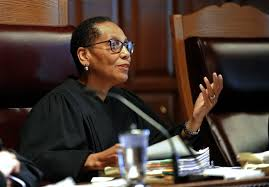
\includegraphics[width=0.3\columnwidth]{../figures/judge}};
          \uncover<2->{
            \node at (-2,-2) (jail) {
\includegraphics[width=0.3\columnwidth]{../figures/jail}};
            \draw[->] (judge) -- (jail);
          }
          \uncover<3->{
            \node at (2,-2) (bail) {
\includegraphics[width=0.3\columnwidth]{../figures/bail}};
            \draw[->] (judge) -- (bail);
          }

          \uncover<4->{
            \node at (-2,-4) (trial) {
\includegraphics[width=0.3\columnwidth]{../figures/trial}};
            \draw[->] (jail) -- (trial);
          }
          \uncover<5->{
            \draw[->] (bail) -- (trial);
          }
          \uncover<6->{
            \node at (2,-4) (arrest) {
\includegraphics[width=0.3\columnwidth]{../figures/handcuffs}};
            \draw[->] (bail) -- (arrest);
          }
        \end{tikzpicture}
      \end{column}
      \begin{column}{0.5\textwidth}
        \centering
        \uncover<7->{
          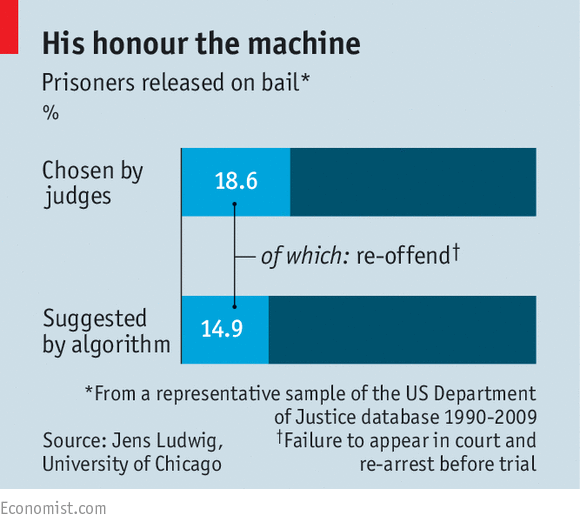
\includegraphics[width=\textwidth]{../figures/judge-fairness}
        }
      \end{column}
    \end{columns}
  }
  
  \only<article>{
    \begin{figure}
      \centering
      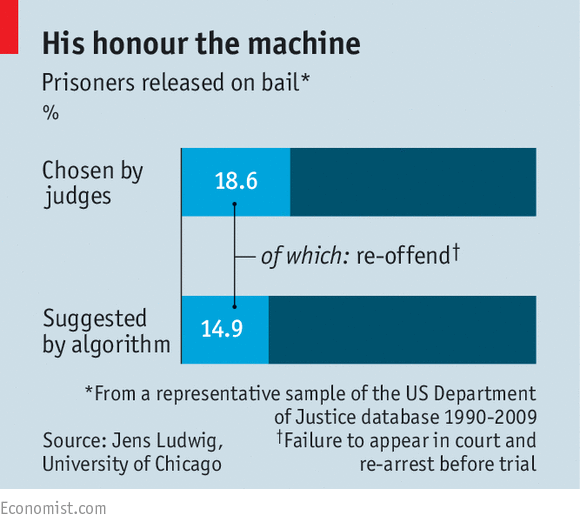
\includegraphics[width=0.5\textwidth]{../figures/judge-fairness}
      \caption{In some cases, it appears as though automating this procedure might lead to better outcomes. But is that generally true?}
      \label{fig:judge-fairness}
    \end{figure}
  }

\end{frame}

\begin{frame}
  \frametitle{Whites get lower scores than blacks\footnote{Pro-publica, 2016}}
  \only<article>{In a different study, it was shown that a commonly used software tool for determining 'risk scores' in the US was biased towards white defendants, who seemed to be always getting lower scores than blacks.}
  \begin{figure}[H]
    \begin{columns}
      \begin{column}{0.5\textwidth}
        \centering
        \def\svgwidth{.95\columnwidth}
        \input{../figures/risk-scores-black.pdf_tex}
        Black
      \end{column}
      \begin{column}{0.5\textwidth}
        \centering
        \def\svgwidth{0.95\columnwidth}
        \input{../figures/risk-scores-white.pdf_tex}      
        White
      \end{column}
    \end{columns}
    \label{fig:risk-bias}
    \caption{Apparent bias in risk scores towards black versus white defendants.}
  \end{figure}
\end{frame}

\begin{frame}
  \frametitle{But scores equally accurately predict recidivsm\footnote{Washington Post, 2016}}
  \only<article>{On the other hand, the scores generated by the software seemed to be very predictive on whether or not defendants would re-offend, independently of their race.}
  \begin{figure}[H]
    \centering
    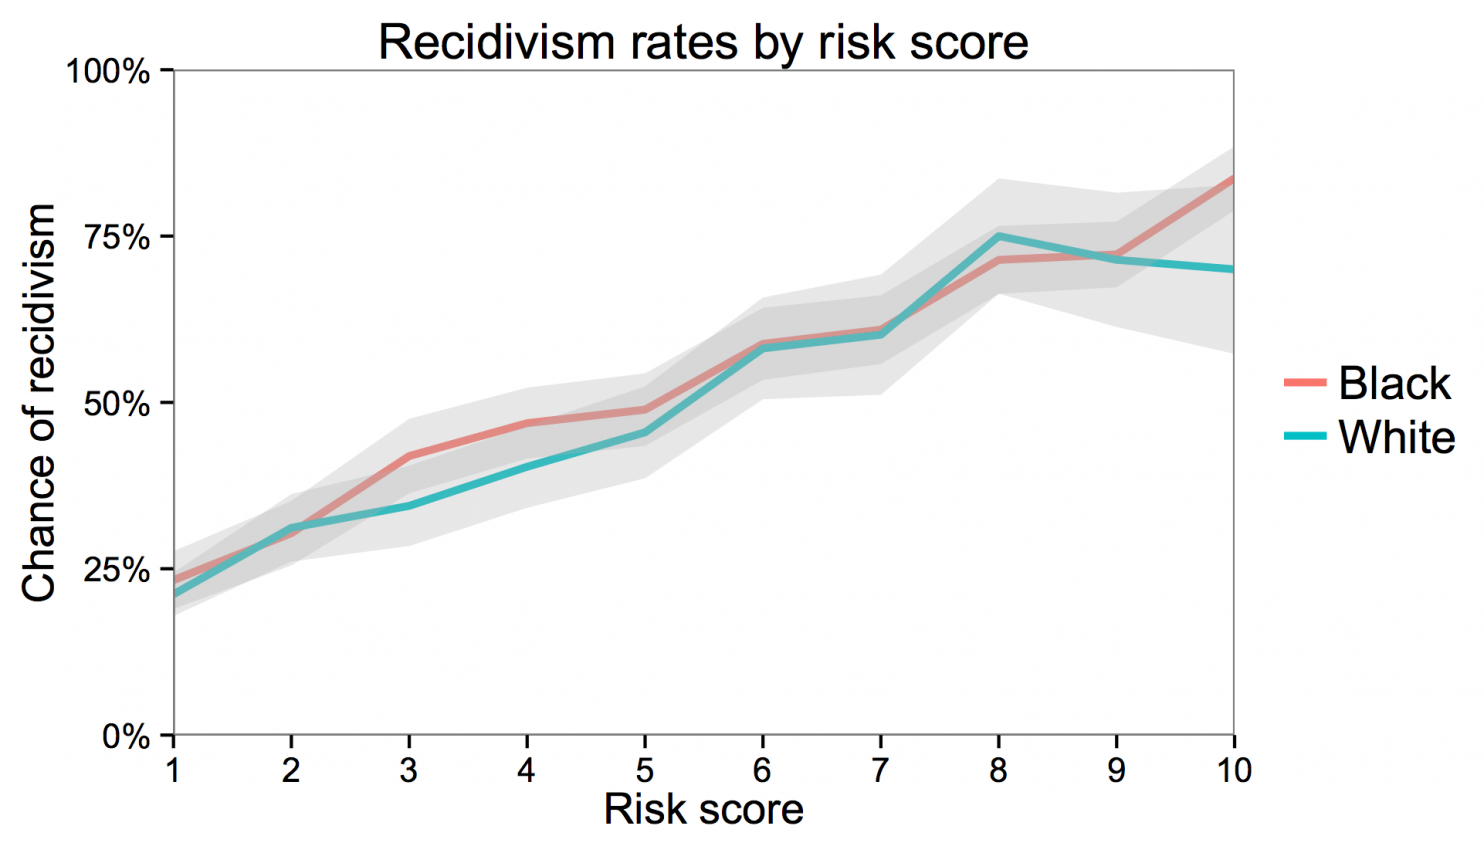
\includegraphics[width=\columnwidth]{../figures/imrs}
    \caption{Recidivism rates by risk score.}
    \label{fig:imrs}
  \end{figure}
\end{frame}
\begin{frame}
  \frametitle{But non-offending blacks get higher scores}
  \only<article>{On the third hand, we see that the system seemed to give higher risk scores to non-offending blacks. So, is there a way to fix that or not?}
  \begin{figure}[H]
    \centering
    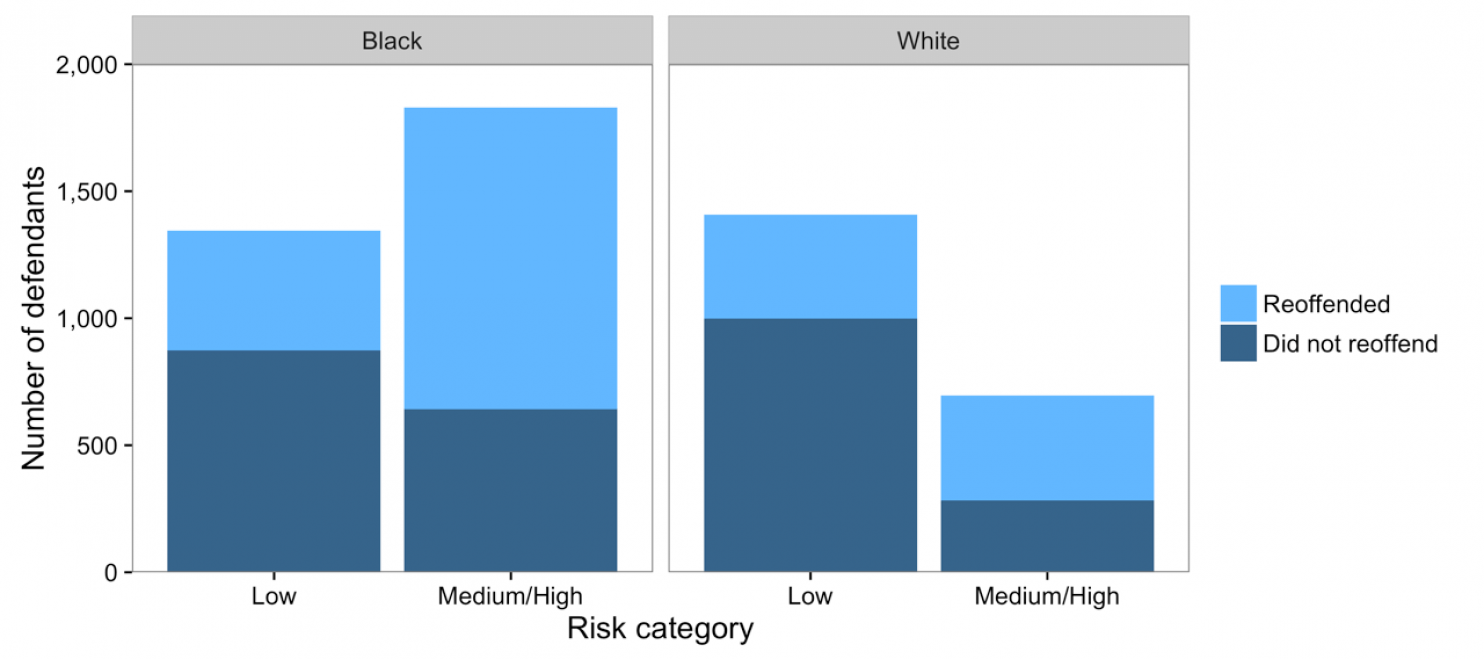
\includegraphics[width=0.95\textwidth]{../figures/imrs-risk}
    \caption{Score breakdown based on recidivism rates.}
    \label{fig:imrs-risk}
  \end{figure}
\end{frame}

\only<presentation>{

  \begin{frame}
    \frametitle{Graphical models and independence}
    \begin{itemize}
    \item Why is it not possible to be fair in all respects?
    \item Different notions of \alert{conditional independence}.
    \item Can only be satisfied rarely simultaneously.
    \end{itemize}
  \end{frame}

}
\only<article>{
  How can we explain this discrepancy? We can show that in fact, each one of these different measures of bias in our decision rules can be seen as a notion of conditional independence. 
}
\only<presentation>{
\section{Graphical models}
\only<article>{
  Graphical models are a very useful tool for modelling the relationship between multiple variables. The simplest such models, probabilistic graphical models (otherwise known as Bayesian networks) involve directed acyclic graphs between random variables. There are two other types of probabilistic models, factor graph and undirected graphical models, which are equivalent to each other, though not to directed models.}
\begin{frame}
  \frametitle{Graphical models}
  \begin{figure}[H]
    \centering
    \begin{tikzpicture}
      \node[RV] at (2,0) (xi) {$x_3$};
      \node[RV] at (0,0) (xB) {$x_1$};
      \node[RV] at (1,1) (xD) {$x_2$};
      \draw[->] (xB) to (xD);
      \draw[->] (xD) to (xi);
      \draw[->] (xB) to (xi);
    \end{tikzpicture}
    \label{fig:bn}
    \caption{Graphical model (directed acyclic graph) for three variables.}
  \end{figure}
  \only<article>{Consider for example the model in Figure~\ref{fig:bn}. It involves three variables, $x_1, x_2, x_3$ and there are three arrows, which show how one variable depends on another. Simply put, if you think of each $x_k$ as a stochastic function, then $x_k$'s value only depends on the values of its parents, i.e. the nodes that are point to it. In this example, $x_1$ does not depend on any other variable, but the value of $x_2$ depends on the value of $x_1$. Such models are useful when we want to describe the joint probability distribution of all the variables in the collection.}
  \begin{block}{Joint probability}
    Let $\bx = (x_1, \ldots, x_n)$. Then $\bx : \Omega \to X$, $X = \prod_i X_i$ and:
    \[
    \Pr(\bx \in A) = P(\cset{\omega \in \Omega}{\bx(\omega) \in A}).
    \]
  \end{block}
  \only<article>{
    When $X_i$ are finite, we can typically write
    \[
    \Pr(\bx = \ba) = P(\cset{\omega \in \Omega}{\bx(\omega) = \ba}),
    \]
    for the probability that $x_i = a_i$ for all $i \in [n]$.
  }
  \begin{block}{Factorisation}
    \only<article>{
      For any subsets $B \subset [n]$ and its complement $C$ so that
      $\bx_B = (x_i)_{i \in B}$,     $\bx_C = (x_i)_{i \notin B}$
    }
    \only<1>{
      \[
      \Pr(\bx) = \Pr(\bx_B \mid \bx_C) \Pr(\bx_C)
      \only<presentation>{,\qquad B, C \subset [n]}
      \]
    }
    \uncover<2->{
      So we can write any joint distribution as
      \[
      \Pr(x_1) \Pr(x_2 \mid x_1) \Pr(x_3 \mid x_1, x_2) \cdots \Pr(x_n \mid x_1, \ldots, x_{n-1}).
      \]
    }
  \end{block}
  \only<article>{Although the above factorisation is always possible to do, sometimes our graphical model has a structure that makes the factors much simpler. In fact, the main reason for introducing graphical models is to represent dependencies between variables. For a given model, we can infer whether some variables are in fact dependent, independent, or conditionally independent.}
\end{frame}
\begin{frame}
  \frametitle{Directed graphical models and conditional independence}
  \begin{figure}[H]
    \centering
    \begin{tikzpicture}
      \node[RV] at (2,0) (xi) {$x_3$};
      \node[RV] at (0,0) (xB) {$x_1$};
      \node[RV] at (1,1) (xD) {$x_2$};
      \draw[->] (xB)--(xD);
      \draw[->] (xD)--(xi);
    \end{tikzpicture}
    \label{fig:bn}
    \caption{Graphical model for the factorisation $\Pr(x_3 \mid x_2) \Pr(x_2 \mid x_1) \Pr(x_1)$.}
  \end{figure}
  \begin{block}{Conditional independence}
    We say $x_i$ is conditionally independent of $\bx_B$ given $\bx_D$ and write $x_i \mid \bx_D \indep \bx_B$ iff
    \[
    \Pr(x_i, \bx_B \mid \bx_D)
    =
    \Pr(x_i \mid \bx_D)
    \Pr(\bx_B \mid \bx_D).
    \]
  \end{block}

  \frametitle{Directed graphical models}
  \only<article>{
    A graphical model is a convenient way to represent conditional independence between variables. There are many variants of graphical models, whose name is context dependent. Other names used in the literature are probabilistic graphical models, Bayesian networks, causal graphs, or decision diagrams. In this set of notes we focus on directed graphical models that depict dependencies between ranom variables.

    \begin{definition}[Directed graphical model] A collection of $n$ random variables $x_i : \Omega \to X_i$, and let $X \defn \prod_i X_i$, with underlying probability measure $P$ on $\Omega$.
      Let $\bx = (x_i)_{i=1}^n$ and for any subset $B \subset[n]$ let
      \begin{align}
        \bx_B &\defn (x_i)_{i \in B}\\
        \bx_{-j} &\defn (x_i)_{i \neq i}
      \end{align}
    \end{definition}
  }
  \only<article>{In a graphical model, conditional independence is represented through directed edges.}


\end{frame}

\begin{frame}
  \begin{example}[Smoking and lung cancer]
    \begin{figure}[H]
      \centering
      \begin{tikzpicture}
        \node[RV] at (0,0) (x1) {$S$};
        \node[RV] at (1,1) (x2) {$C$};
        \node[RV] at (2,0) (x3) {$A$};
        \draw[->] (x1)--(x2);
        \draw[->] (x3)--(x2);
      \end{tikzpicture}
      \caption{Smoking and lung cancer graphical model, where $S$: Smoking, $C$: cancer, $A$: asbestos exposure.}
    \end{figure}
    \only<article>{
      It has been found by~\citet{lee2001relation} that lung  incidence not only increases with both asbestos exposure and smoking. This is in agreement with the graphical model shown. The study actually found that there is an amplification effect, whereby smoking and asbestos exposure increases cancer risk by 28 times compared to non-smokers. This implies that the risk is not simply additive. The graphical model only tells us that there is a dependency, and does not describe the nature of this dependency precisely.}
  \end{example}
  \begin{block}{Explaining away}
    Even though $S, A$ are independent, they become dependent once you know $C$. \only<article>{For example, let us say we know that you have cancer and that our model says that it's very unlikely to have cancer unless you either smoke or are exposed to asbestos. When we also learn that you do not have asbestos exposure, smoking becomes more likely. In either words, if cancer is caused by either smoking or asbestos, and we rule out asbestos, the only remaining explanation is smoking. This is what is generally called \alert{explaining away.}}
  \end{block}
\end{frame}

\begin{frame}
  \begin{example}[Time of arrival at work]
    \begin{figure}[H]
      \centering
      \begin{tikzpicture}
        \node[RV] at (0,0) (x1) {$x_1$};
        \node[RV] at (1,1) (x2) {$T$};
        \node[RV] at (2,0) (x3) {$x_2$};
        \draw[->] (x2)--(x3);
        \draw[->] (x2)--(x1);
      \end{tikzpicture}
      \caption{Time of arrival at work graphical model where $T$ is a traffic jam and $x_1$ is the time John arrives at the office and $x_2$ is the time Jane arrives at the office.}
    \end{figure}
    \only<article>{
      In this model, the arrival times of John and Jane may seem correlated. However, there is a common cause: The existence of a traffic jam. Whenever there is a traffic jam, both John and Jane are usually late. Whenever there is not a traffic jam, they are both mostly on time.
    }
  \end{example}
  \begin{block}{Conditional independence}
    Even though $x_1, x_2$ are correlated, they become independent once you know $T$.
  \end{block}
\end{frame}

\begin{frame}
  \begin{example}[Treatment effects]
    \begin{figure}[H]
      \centering
      \begin{tikzpicture}
        \node[RV] at (0,0) (x) {$x$};
        \node[RV] at (1,1) (y) {$y$};
        \node[RV] at (2,0) (a) {$a$};
        \draw[->] (x)--(y);
        \draw[->] (x)--(a);
        \draw[->] (a)--(y);
      \end{tikzpicture}
      \caption{Kidney treatment model, where $x$: severity, $y$: result, $a$: treatment applied}
    \end{figure}
    \begin{table}[H]
      \begin{tabular}{l|r|r}
        & Treatment A  & Treatment B\\
        \hline
        Small stones & 87  & 270\\
        Large stones  & 263 &  80
      \end{tabular}
      \begin{tabular}{l|r|r}
        Severity & Treatment A  & Treatment B\\
        \hline
        Small stones ) & 93\%  & 87\%\\
        Large stones  & 73\% &  69\%\\
        \hline
        Average & 78\% & 83\%
      \end{tabular}
    \end{table}
    \only<article>{
       A curious example is that of applying one of two treatments for kidneys. In the data, it is clear that one treatment is best for both large and small stones. However, when the data is aggregated it appears as though treatment B is best. This is because treatment A is chosen much more frequently when the stones are large, and that's when both treatments perform worse. This apparent discrepancy is called \emph{Simpson's paradox}\index{Simpson's paradox}}
  \end{example}
\end{frame}


\begin{frame}
  \begin{example}[School admission]
    \begin{figure}[H]
      \centering
      \begin{subfigure}{0.45\textwidth}
        \begin{tikzpicture}
          \node[RV] at (0,0) (z) {$z$};
          \node[RV] at (1,1) (s) {$s$};
          \node[RV] at (2,0) (a) {$a$};
          \draw[->] (z)--(s);
          \draw[->] (z)--(s);
          \draw[->] (s)--(a);
        \end{tikzpicture}
      \end{subfigure}
      \begin{subfigure}{0.45\textwidth}
        \begin{tikzpicture}
          \node[RV] at (0,0) (z) {$z$};
          \node[RV] at (1,1) (s) {$s$};
          \node[RV] at (2,0) (a) {$a$};
          \draw[->] (z)--(s);
          \draw[->] (z)--(s);
          \draw[->] (s)--(a);
          \draw[->] (z)--(a);
        \end{tikzpicture}
      \end{subfigure}
      \caption{School admission graphical model, where $z$: gender, $s$: school applied to, $a$: whether you were admitted. }
    \end{figure}
    \begin{table}[H]
      \begin{tabular}{l|r|r}
        School & Male  & Female\\
        \hline
        A & 62\% & 82\%\\
        B & 63\% & 68\%\\
        C & 37\% & 34\%\\
        D & 33\% & 35\%\\
        E & 28\% & 24\%\\
        F &  6\% &  7\%\\
        \hline
        \emph{Average} & \emph{45\%} & \emph{38\%}
      \end{tabular}
    \end{table}
    \only<article>{In this example, it appears as though female candidates have a lower acceptance rate than males. However what is missing is the fact that many more males are applying to easier schools. Thus, it is possible that the data is explainable by the fact that admission only reflects the difficulty of each school, and the overall gender imbalance is due to the choices made by the applicants. However, an alternative model is that the admissions process also explicitly takes gender into account. However, both of these models may be inadequate, as we do not have data about each individual applicant, such as their grades. We shall discuss this issue further when we talk about causality, confounding variables and counterfactuals.}
  \end{example}
\end{frame}


\begin{frame}
  \begin{exercise}
    Factorise the following graphical model.
    \centering
    \begin{tikzpicture}
      \node[RV] at (0,0) (x1) {$x_1$};
      \node[RV] at (1,-1) (x2) {$x_2$};
      \node[RV] at (1,1) (x3) {$x_3$};
      \node[RV] at (2,0) (x4) {$x_4$};
      \draw[->] (x1)--(x2);
      \draw[->] (x1)--(x3);
    \end{tikzpicture}
  \end{exercise}
  \uncover<2>{
    \[
    \Pr(\bx)
    = \Pr(x_1) \Pr(x_2 \mid x_1) \Pr(x_3 \mid x_1) \Pr(x_4)
    \]
  }

\end{frame}

\begin{frame}
  \begin{exercise}
    Factorise the following graphical model.
    \centering
    \begin{tikzpicture}
      \node[RV] at (0,0) (x1) {$x_1$};
      \node[RV] at (1,-1) (x2) {$x_2$};
      \node[RV] at (1,1) (x3) {$x_3$};
      \node[RV] at (2,0) (x4) {$x_4$};
      \draw[->] (x1)--(x2);
      \draw[->] (x1)--(x3);
      \draw[->] (x3)--(x4);
    \end{tikzpicture}
  \end{exercise}
  \uncover<2>{
    \[
    Xb      \Pr(\bx)
    = \Pr(x_1) \Pr(x_2 \mid x_1) \Pr(x_3 \mid x_1) \Pr(x_4 \mid x_3)
    \]
  }

\end{frame}

\begin{frame}
  \begin{exercise}
    What dependencies does the following factorisation imply?
    \[
    \Pr(\bx)
    = \Pr(x_1) \Pr(x_2 \mid x_1) \Pr(x_3 \mid x_1) \Pr(x_4 \mid x_2, x_3)
    \]
    \centering
    \begin{tikzpicture}
      \node[RV] at (0,0) (x1) {$x_1$};
      \node[RV] at (1,-1) (x2) {$x_2$};
      \node[RV] at (1,1) (x3) {$x_3$};
      \node[RV] at (2,0) (x4) {$x_4$};
      \uncover<2>{
        \draw[->] (x1)--(x2);
        \draw[->] (x1)--(x3);
        \draw[->] (x3)--(x4);
        \draw[->] (x2)--(x4);
      }
    \end{tikzpicture}
  \end{exercise}
\end{frame}


%%% Local Variables:
%%% mode: latex
%%% TeX-master: "notes"
%%% End:




\begin{frame}
  \begin{alertblock}{Deciding conditional independence}
    There is an algorithm for deciding conditional independence of any two variables in a graphical model.
    \only<article>{However, this is beyond the scope of these notes. Here, we shall just use these models as a way to encode dependencies that we assume exist.}
  \end{alertblock}

\end{frame}

\subsection{Inference and prediction in graphical models}
\begin{frame}
\frametitle{Inference and prediction in graphical models}
 \begin{figure}[H]
     \centering
     \begin{tikzpicture}
       \node[RV, hidden] at (0,0) (param) {$\param$};
       \node[RV] at (-1,1) (data1) {$x_1$};
       \node at (0,1) (data2) {$\cdots$};
       \node[RV] at (1,1) (data3) {$ x_t$};
       \draw[->] (param)--(data1);
       \draw[->] (param)--(data3);
       \node<2->[RV] at (2,1) (new_data) {$x_{t+1}$};
       \draw<2->[->] (param)--(new_data);
     \end{tikzpicture}
     \caption{Inference and prediction in a graphical model}. 
   \end{figure}
\only<article>{In this example, $x_1, \ldots, x_t$ are all i.i.d, drawn from the distribution $P_\param(x_t) = \Pr(x_t \mid \param)$.}
  \only<1>{
    \begin{block}{Inference of latent variables}\index{inference}
      \[
      \Pr(\param \mid x_1, \ldots, x_t)
      \]
      \only<article>{Inference in graphical models typically refers to the problem of estimating the distribution of some \emph{hiddeen} or \emph{latent} variable from data. These variables are generally thought of as two types:}
      \begin{itemize}
      \item Model parameters. \only<article>{These generally do not change over time. One example is estimating the mean of a Gaussian distribution from data.}
      \item System states. \only<article>{These typically are time-indexed. We will see further examples of such variables when we discuss latent variable models. On example is inferring location from GPS measurements.} 
      \end{itemize}
    \end{block}
  }
  \only<2>{
    \begin{block}{Prediction}\index{prediction}
      \[
      \Pr(x_{t+1} \mid x_1, \ldots, x_t)
      =
      \int_\Param \Pr(x_{t+1} \mid \param) \dd \Pr(\param \mid x_1, \ldots, x_t)
      \]
      \only<article>{Prediction is a type of inference, but differs in that the variable whose distribution we wish to estimate is only temporarily not observed: we can actually obtain its value in the future. Thus, a prediction is always testable!}
      \only<presentation>{
        Predictions are \alert{testable.}
      }
    \end{block}
  }
\end{frame}

\begin{frame}
\frametitle{Coin tossing, revisited}
\begin{example}{The Beta-Bernoulli prior}
  \begin{figure}[H]
    \centering
    \begin{tikzpicture}
      \node[RV] at (0,0) (bel) {$\bel$}; \node[RV, hidden] at (1,0)
      (param) {$\param$}; \node[RV] at (2,0) (data) {$x$}; \draw[->]
      (bel)--(param); \draw[->] (param)--(data);
    \end{tikzpicture}
    \caption{Graphical model for a Beta-Bernoulli prior}
  \end{figure}
  \begin{align}
    \param &\sim \BetaDist(\bel_1, \bel_2), && \textrm{i.e.  $\bel$ are Beta distribution parameters}\\
    x \mid \param &\sim \Bernoulli(\param), && \textrm{i.e. $P_\param(x)$ is a Bernoulli}
  \end{align}
  \only<article>{In this example, it is obvious why we use the notation above for describing hierarchical models.\index{hierarchical Bayesian model} We simply state what is the distribution on one variable conditioned on the other variables. Here, $\bel$ is fixed, and it is something we can choose arbitrarily. The data $x$ is observed, while the parameter $\param$ remains \emindex{latent}. Using Bayes theorem, we can derive the distribution for $\bel(\theta \mid x)$. In this particular case, we elide referring to a sample $x_1. \ldots, x_t$ as they are all i.i.d.}
\end{example}
\end{frame}

\begin{frame}
  \begin{example}{The $n$-meteorologists problem (continuation of Exercise~\ref{ex:meteorologists})}\index{$n$-meteorologists}
    \only<presentation>{
      \begin{itemize}
      \item Meteorological models $\CM = \set{\model_1, \ldots, \model_n}$
      \item Rain predictions at time $t$: $p_{t,\model} \defn  P_{\model}(x_t = \textrm{rain})$.
      \item Prior probability $\bel(\model) = 1/n$ for each model.
      \item Decision $a$, resulting in utility $\util(a, x_{t+1})$
      \end{itemize}
    }
    \begin{figure}[H]
      \centering
      \begin{tikzpicture}
        \node[RV] at (0,-1) (bel) {$\bel$};
        \node[RV, hidden] at (0,0) (param) {$\model$};
        \node[RV] at (-1,1) (data1) {$x_1$};
        \node at (0,1) (data2) {$\cdots$};eu
        \node[RV] at (1,1) (data3) {$ x_t$};
        \draw[->] (param)--(data1);
        \draw[->] (param)--(data3);
        \node[RV] at (2,1) (new_data) {$x_{t+1}$};
        \draw[->] (param)--(new_data);
        \draw[->] (bel)--(param);
        \node[select] at (2,-1) (act) {$a$};
        \node[utility] at (4,-1) (util) {$\util$};
        \draw[->] (act)--(util);
        \draw[->] (new_data)--(util);
        \draw[->] (data3)--(new_data);
        \draw[->] (data1) to [bend left] (new_data);
        \draw[->] (data1) to [bend right] (data3);
      \end{tikzpicture}
     \caption{Inference, prediction and decisions in a graphical model.}
   \end{figure}
   \only<article>{In this problem, we allow each model's predictions to have arbitrary dependences with the past i.e.
     \[
     P_\model(x_{t+1} \mid x_t, x_{t-1}, \ldots, x_1).
     \]
     For inference, the details of how each model works are not important: just the probability of the next observation given the previous ones.
   }
  \end{example}


\end{frame}


\subsection{Testing conditional independence}
\begin{frame}
  \frametitle{Measuring independence}
  \only<article>{The simplest way to measure independence is by looking at whether or not the distribution of the possibly dependent variable changes when we change the value of the other variables. }

  \begin{theorem}
    If $x_i \mid \bx_D \indep \bx_B$ then
    \[
    \Pr(x_i \mid \bx_B, \bx_D)
    =
    \Pr(x_i \mid \bx_D)
    \]
  \end{theorem}
  \uncover<2->{
    This implies
    \[
    \Pr(x_i \mid \bx_B = b, \bx_D)
    =
    \Pr(x_i \mid \bx_B = b', \bx_D)
    \]
    so we can measure independence by seeing how the distribution of $x_i$ changes when we vary $\bx_B$, keeping $\bx_D$ fixed.
  }
    \only<article>{For any given model, there is either a dependence or there is not. However, sometimes we might be able to tolerate some amount of dependence. Thus, we can simply measure the deviation from independence through a metric or divergence on distributions.}
  \begin{example}
    \[
    \|\Pr(a \mid y, z) - \Pr(a \mid y)\|_1
    \]
    which for discrete $a,y,z$ is:
    \[
    \max_{i,j} \|\Pr(a \mid y = i, z = j) - \Pr(a \mid y= i)\|_1
    =
    \max_{i,j} \|\sum_k \Pr(a = k \mid y = i, z = j) - \Pr(a =k \mid y= i)\|_1.
    \]
    See also \url{src/fairness/ci_test.py}
  \end{example}
\end{frame}


\begin{frame}
\begin{example}{An alternative model for coin-tossing}
  This is an elaboration of Example~\ref{ex:bayesian-compound-hypothesis-test} for hypothesis testing.
  \begin{figure}[H]
    \centering
    \begin{tikzpicture}
      \node[RV] at (-1,0) (hbel) {$\hyperparam$};
      \node[RV] at (1,1) (bel) {$\bel$};
      \node[RV, hidden] at (0,0) (model) {$\model$};
      \node[RV, hidden] at (1,0) (param) {$\param$};
      \node[RV] at (2,0) (data) {$x$};
      \draw[->] (hbel)--(model);
      \draw[->] (bel)--(param);
      \draw[->] (model)--(param);
      \draw[->] (param)--(data);
    \end{tikzpicture}
    \caption{Graphical model for a hierarchical prior}
  \end{figure}
  \begin{itemize}
  \item $\model_1$: A Beta-Bernoulli model with $\BetaDist(\bel_1, \bel_2)$
  \item $\model_0$: The coin is fair.
  \end{itemize}
  \begin{align}
    \param \mid \model = \model_0 &\sim \Singular(0.5), && \textrm{i.e. $\param$ is always 0.5}\\
    \param \mid \model = \model_1 &\sim \BetaDist(\bel_1, \bel_2), && \textrm{i.e. $\param$ has a Beta distribution}\\
    x \mid \param &\sim \Bernoulli(\param), && \textrm{i.e. $P_\param(x)$ is Bernoulli}
  \end{align}
  Here the posterior over the two models is simply
  \[
  \hyperparam(\model_0 \mid x) = \frac{P_{0.5}(x) \hyperparam(\model_0)}{P_{0.5}(x) \hyperparam(\model_0) + \Pr_{\model_1}(x) \hyperparam(\model_1)},
  \qquad
  \Pr_{\model_1(x)} = \int_0^1 P_\param(x) \dd \bel(\param).
  \]
\end{example}

\end{frame}

\begin{frame}
  \frametitle{Bayesian testing of independence}
  \only<article>{
    For a given distributional model $P_\param$, conditional independence either holds or does not. Consider the set of model parameters $\Param_0$ where, for each parameter $\param \in \Param_0$, we have a conditional independence condition, while $\Param_1$ may corresponds to models where there may not be independence. To make this more concrete, let's give an example.}

    \begin{figure}[H]
      \centering
      \begin{subfigure}[b]{0.45\textwidth}
        \begin{tikzpicture}
          \node[RV] at (0,0) (x1) {$x_1$};
          \node[RV] at (1,1) (x2) {$x_2$};
          \node[RV] at (2,0) (x3) {$x_3$};
          \draw[->] (x1)--(x2);
          \draw[->] (x2)--(x3);
        \end{tikzpicture}
        \caption{$\Param_0$ assumes independence}
      \end{subfigure}
     \begin{subfigure}[b]{0.45\textwidth}
     \begin{tikzpicture}
        \node[RV] at (0,0) (x1) {$x_1$};
        \node[RV] at (1,1) (x2) {$x_2$};
        \node[RV] at (2,0) (x3) {$x_3$};
        \draw[->] (x1)--(x2);
        \draw[->] (x2)--(x3);
        \draw[alert,->] (x1)--(x3);
      \end{tikzpicture}
      \caption{$\Param_1$ does \alert{not} assume independence}
    \end{subfigure}
    \only<article>{\caption{The two alternative models}}
    \end{figure}
  \begin{example}
    \only<1>{
    Assume data $D = \cset{x^t_1, x^t_2, x^t_3}{t = 1, \ldots, T}$ with $x_i^t \in \set{0,1}$.
    \only<article>{First consider model $\Param_0$ where the following conditional independence holds
    \[
    P_\param(x_3 \mid x_2, x_1) = P_\param(x_2 \mid x_1), \qquad \forall \param \in \Param_0.
    \]
    In the alternative model $\Param_1$ there is no
      independence assumption. So the likelihood for either a model in either set is}
    \begin{align}
    P_\param(D) &= \prod_t P_\param(x^t_3 \mid x^t_2) P_\param(x^t_2 \mid x^t_1) P_\param(x^t_1), \qquad \param \in \Param_0\\
    P_\param(D) &= \prod_t P_\param(x^t_3 \mid x^t_2, \alert{x_1^t}) P_\param(x^t_2 \mid x^t_1) P_\param(x^t_1), \qquad \param \in \Param_1
    \end{align}
  }
  \only<2>{
    \only<article>{The parameters for this example can be defined as follows}
    \begin{align}
      \param_1 &\defn P_\param(x^t_1 = 1) \tag{$\model_0,\model_1$}\\
      \param_{2|1}^{i} &\defn P_\param(x^t_2 = 1 \mid x^t_1 = i) \tag{$\model_0, \model_1$}\\
      \param_{3|2}^{j} &\defn P_\param(x^t_3 = 1 \mid x^t_2 = j) \tag{$\model_0$}\\
      \param_{3|2,1}^{i,j} &\defn P_\param(x^t_3 = 1\mid x^t_2=j, x_1^t=i)\tag{$\model_1$}
    \end{align}
    \only<article>{
      We model each one of these parameters with a separate Beta-Bernoulli distribution.
    }
  }
  \end{example}

\end{frame}



\subsection{Hierarchical Bayesian models}
\begin{frame}
\only<article>{Given some data $D$, the Bayesian approach would involve specifying a hierarchical prior\index{hierarchical Bayesian model} $\bel$ so that $\hyperparam(\model_1) = 1 - \hyperparam(\model_0)$ specifies a probability on the two model structures, while for the $i$-th model we define a prior $\bel_i(\param)$ over $\Param_i$, so that we obtain the following hierarchical model
  }
  \begin{figure}[H]
    \centering
    \begin{tikzpicture}
      \node[RV, hidden] at (0,0) (model) {$\model$};
      \node[RV, hidden] at (1,0) (param) {$\param$};
      \node[RV] at (2,0) (data) {$D$};
      \draw[->] (model)--(param);
      \draw[->] (param)--(data);
    \end{tikzpicture}
        \caption{Hierarchical model.}
    \label{fig:hierarchical-model}
  \end{figure}
\only<article>{Here the specific model $\model$ is unobserved, as well as its parameters $\param$. Only the data $D$ is observed. Our prior distribution is omitted from the graph.}
\only<1>{
\begin{align}
  \model_i &\sim \hyperparam\\
  \param \mid \model = \model_i &\sim \bel_i
\end{align}
}
\only<1->{
  \begin{block}{Marginal likelihood}
    \only<article>{This gives the the following marginal likelihood for the combined models and each of the models respectively.}
    \begin{align}
      \Pr_\hyperparam(D) &= \hyperparam(\model_0) \Pr_{\model_0}(D)  + \hyperparam(\model_1) \Pr_{\model_1}(D)\\
      \Pr_{\model_i}(D) &= \int_{\Param_{i}} P_{\param}(D) \dd \bel_i(\param).
    \end{align}
  \end{block}
}
\only<2->{
  \begin{block}{Model posterior}
    \begin{equation}
      \hyperparam(\model \mid D) = 
      \frac{\Pr_\model(D) \hyperparam(\model)}
      {\sum_{i} \Pr_{\model_i} (D) \hyperparam(\model_i)}
    \end{equation}
  \end{block}
}
\end{frame}

\begin{frame}
  \frametitle{Calculating the marginal likelihood}
  \only<article>{Generally speaking, calculating the marginal likelihood for a model with an uncountable parameter set is hard. However, conjugate models admit closed form solutions and efficient calculations. Firstly, let's rewrite the marginal likelihood in terms of an integral Monte-Carlo approximation.}
  \begin{block}{Monte-Carlo approximation}
    \begin{align}
      \label{eq:mc-marginal-likelihood}
      \int_\Param P_\param(D) \dd \bel(\param)
      &\approx
        \sum_{n=1}^N P_{\param_n}(D)  + O(1/\sqrt{N}), & \param_n &\sim \bel
    \end{align}
  \end{block}
  \only<article>{Even though this approximation is reasonable at first glance, the problem is that the leading constant of the error scales approximately proportionally to the maximum likelihood $\max_\param P_\param(D)$. This is a consequence of Hoeffding's inequality~\eqref{eq:Hoeffding}. Thus, the more data we have the more samples we need to get a good approximation with this simple Monte Carlo approach. For that reason, one typically uses a sample from a proposal distribution $\psi$ which is different from $\bel$. Then it holds}
  \begin{block}{Importance sampling}
    \only<article>{For any two measures $\bel, \psi$ on $\Param$, we can write:}
    \index{importance sampling}
    \begin{align}
      \label{eq:importance-sampling}
      \int_\Param P_\param(D) \dd \bel(\param)
      &
        \only<2>{
        =
        \int_\Param P_\param(D) \frac{\dd \psi(\param)}{\dd \psi(\param)} \dd \bel(\param)
        }
        \only<3>{
        =
        \int_\Param P_\param(D) \frac{\dd \bel(\param)}{\dd \psi(\param)} \dd \psi(\param)
        }
        \uncover<4>{
        \approx
        \sum_{n=1}^N P_\param(D) \frac{\dd \bel(\param_n)}{\dd \psi(\param_n)}, & \param_n \sim \psi
        }
    \end{align}
    \only<article>{This allows us to estimate the marginal likelihood with respect to a belief $\bel$ by sampling from an alternative belief $\psi$.}
  \end{block}
\end{frame}

\begin{frame}
  \begin{block}{Sequential updating of the marginal likelihood}
    \begin{align}
      \label{eq:sequential-likelihood}
      \Pr_\bel(D)
      \uncover<2->{
      &= \Pr_\bel(x_1, \ldots, x_T) 
        }
      \uncover<3->{
      \\
      & = \Pr_\bel(x_2, \ldots, x_T \mid x_1) \Pr_\bel(x_1)
        }
      \uncover<4->{
      \\
      & = \alert{\prod_{t=1}^T \Pr_\bel(x_t \mid x_1, \ldots, x_{t-1})}
        }
        \uncover<5->{
      \\
      & = \prod_{t=1}^T \int_\Param P_{\param_n}(x_t) \dd \underbrace{\bel(\param \mid x_1, \ldots, x_{t-1})}_{\textrm{posterior at time $t$}}
        }
    \end{align}
    \only<article>{The nice thing about this break down is that for a simple model such as Beta-Bernoulli, the individual datapoint marginal likelihoods are easy to compute}
  \end{block}
  \begin{example}[Beta-Bernoulli]
    \only<article>{The marginal predictive distribution for a Beta-Bernoulli prior is}
    \index{hierarchical Bayesian model, Beta-Bernoulli}
    \[\Pr_\bel(x_t = 1 \mid x_1, \ldots, x_{t-1}) = \frac{\alpha_t}{\alpha_t + \beta_t},
    \]
    with
    $\alpha_t = \alpha_0 + \sum_{n=1}^{t-1} x_n, \quad \beta_t = \beta_0 + \sum_{n=1}^{t-1} (1 - x_n)$
  \end{example}
\end{frame}
\begin{frame}
  \frametitle{Further reading}
  \begin{block}{Python sources}
    \begin{itemize}
    \item A simple python measure of conditional independence \url{src/fairness/ci_test.py}
    \item A simple test for discrete Bayesian network \url{src/fairness/DirichletTest.py}
    \item Using the PyMC package \url{https://docs.pymc.io/notebooks/Bayes_factor.html} 
    \end{itemize}
  \end{block}
\end{frame}

%%% Local Variables:
%%% mode: latex
%%% TeX-engine: xetex
%%% TeX-master: "notes"
%%% End:

}



\section{Concepts of fairness}
\begin{frame}
  \frametitle{Bail decisions, revisited}
  \only<article>{Let us think of this problem in terms of bail decisions made by a judge using some policy $\pol$ with $\pol(a \mid x)$ being the probability that the judge decides $a$ when she observes $x$. Let $y$ be the outcome, which may or may not depend on $a$. In this particular case, $a$ is either release or jail. And $y$ is appears for trial or not. If we accept the tenets of decision theory, there is also a utility function $U(a, y)$ defined on which the judge bases her decision.}
  \only<presentation>{
    \centering

    \begin{columns}
      \begin{column}{0.5\textwidth}
        \begin{tikzpicture}
          \node[label=$x$] at (-1,2) (person)
          {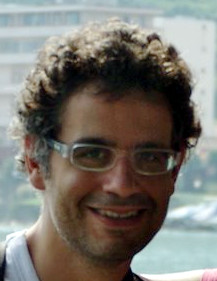
\includegraphics[width=0.2\columnwidth]{../figures/me-recent}};
          \node[label=$\pi$] at (0,0) (judge) {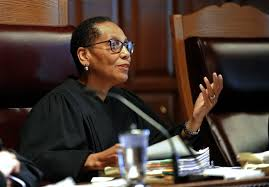
\includegraphics[width=0.3\columnwidth]{../figures/judge}};
          \draw[->] (person) -- (judge);
          \uncover<2->{
            \node[label=$a_1$] at (-2,-2) (jail) {
\includegraphics[width=0.3\columnwidth]{../figures/jail}};
            \draw[->] (judge) -- (jail);
          }
          \uncover<3->{
            \node[label=$a_2$] at (2,-2) (bail) {
\includegraphics[width=0.3\columnwidth]{../figures/bail}};
            \draw[->] (judge) -- (bail);
          }
          \uncover<4->{
            \node[label=$y_1$] at (-2,-4) (trial) {
\includegraphics[width=0.3\columnwidth]{../figures/trial}};
            \draw[->] (jail) -- (trial);
          }
          \uncover<5->{
            \draw[->] (bail) -- (trial);
          }
          \uncover<6->{
            \node[label=$y_2$] at (2,-4) (arrest) {
\includegraphics[width=0.3\columnwidth]{../figures/handcuffs}};
            \draw[->] (bail) -- (arrest);
          }
        \end{tikzpicture}
      \end{column}
      \begin{column}{0.5\textwidth}
        \uncover<2->{\[\pi(a \mid x) \tag{policy}\]}
        \uncover<4->{\[\Pr(y \mid a, x) \tag{outcome}\]}
        \uncover<7->{\[U(a,y) \tag{utility}\]}
      \end{column}
    \end{columns}
  }
  \only<article>{
    \begin{figure}[H]
      \centering
      \begin{tikzpicture}
        \node[label=$x$] at (-1,3) (person)
        {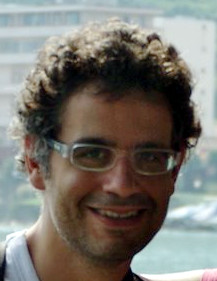
\includegraphics[width=0.1\textwidth]{../figures/me-recent}};
        \node[label=$\pi$] at (0,0) (judge) {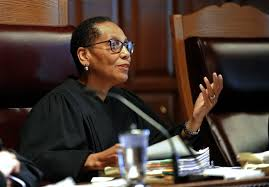
\includegraphics[width=0.2\textwidth]{../figures/judge}};
        \draw[->] (person) -- (judge);
        \uncover<2->{
          \node[label=$a_1$] at (-2,-3) (jail) {
\includegraphics[width=0.2\textwidth]{../figures/jail}};
          \draw[->] (judge) -- (jail);
        }
        \uncover<3->{
          \node[label=$a_2$] at (2,-3) (bail) {
\includegraphics[width=0.2\textwidth]{../figures/bail}};
          \draw[->] (judge) -- (bail);
        }
        \uncover<4->{
          \node[label=$y_1$] at (-2,-6) (trial) {
\includegraphics[width=0.2\textwidth]{../figures/trial}};
          \draw[->] (jail) -- (trial);
        }
        \uncover<5->{
          \draw[->] (bail) -- (trial);
        }
        \uncover<6->{
          \node[label=$y_2$] at (2,-6) (arrest) {
\includegraphics[width=0.2\textwidth]{../figures/handcuffs}};
          \draw[->] (bail) -- (arrest);
        }
      \end{tikzpicture}
      \caption{The bail decision process, simplified.}
      \label{fig:bail-process}
    \end{figure}
  }
\end{frame}


\subsection{Fairness as independence}
\begin{frame}
  \only<article>{So how can we reframe the above fairness notions in a more precise way? Both of them involve conditional independence between $y, a$ and a sensitive attribute $z$, such as race. The first notion says that the actions of the judge (or equivalently, the scores of the algorithm) are \emph{calibrated} with respect to the outcomes. The second says that they are \emph{balanced}, so that were the outcome known to the judge, she would be making a decision independently of the defendant's race. Both of these conditions were discussed in a more restricted setting by }
  \only<presentation>{
    \only<1>{
      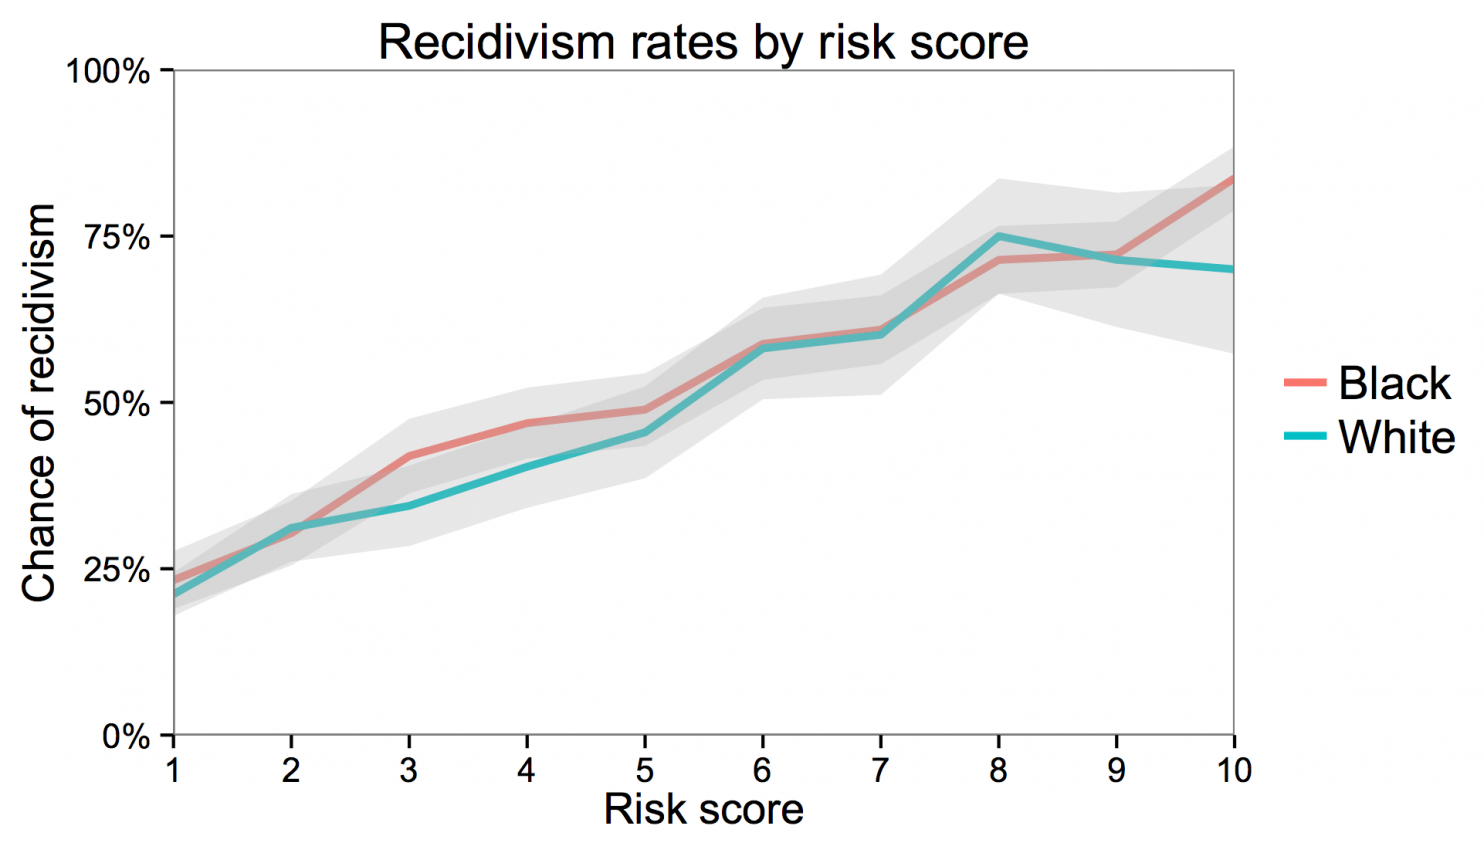
\includegraphics[width=\columnwidth]{../figures/imrs}
    }
    \only<2>{
      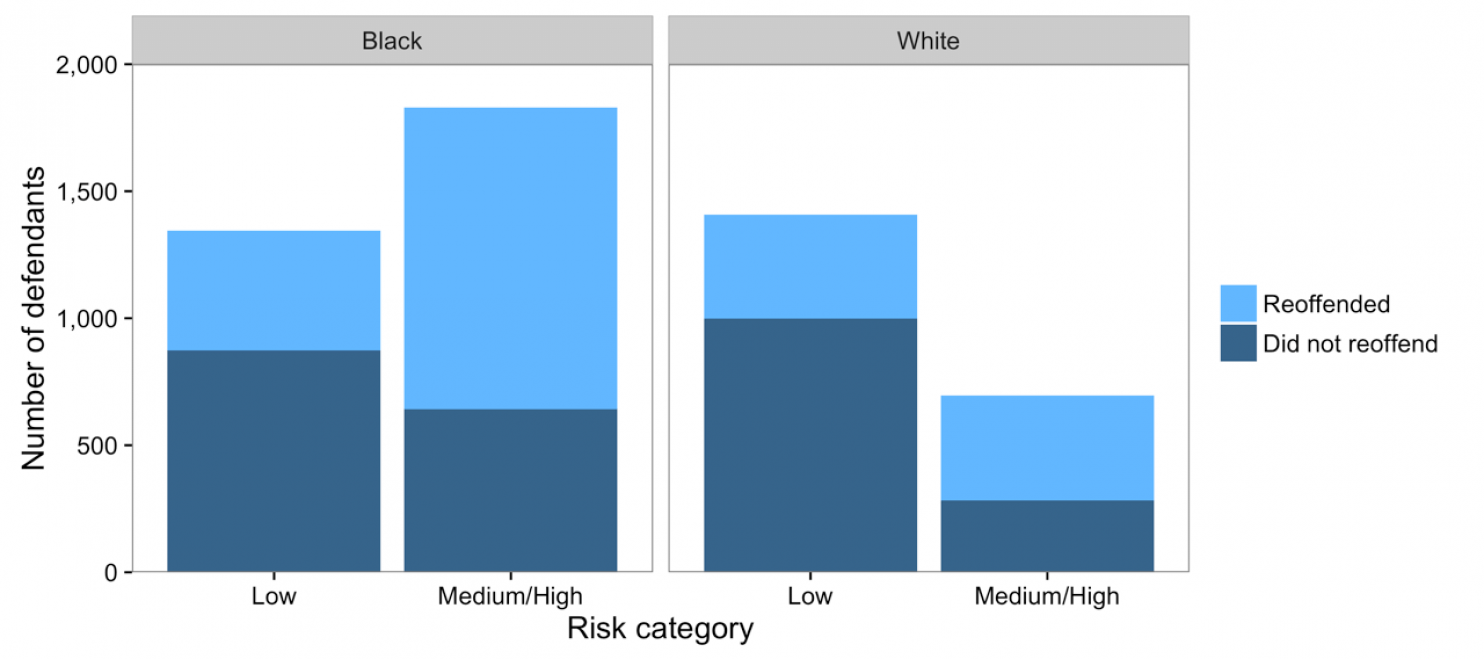
\includegraphics[width=\columnwidth]{../figures/imrs-risk}
    }
    \begin{columns}
      \begin{column}{0.3\textwidth}
        \begin{itemize}
        \item[$y$] Result.
        \item[$a$] Assigned score.
        \item[$z$] Race.
        \end{itemize}
      \end{column}
      \begin{column}{0.7\textwidth}
        \begin{align}
          \Pr^\pi(y \mid a, z) &= \Pr^\pi(y \mid a) \tag{\alert<1>{calibration}}\\
          \Pr^{\pi}(a \mid y, z) &= \Pr^{\pi}(a \mid y) \tag{\alert<2>{balance}}
        \end{align}
      \end{column}
    \end{columns}
  }
  \only<article>{
    \begin{definition}[Calibration]
      A policy $\pol$ is calibrated for parameter $\param$ with respect to $z$ if
      \begin{equation}
        \Pr_\param^\pol(y \mid a, z) = \Pr_\param^\pol(y \mid a), \qquad \forall a, z.
        \label{eq:calibration}
      \end{equation}
    \end{definition}
    You will observe that calibration here means that
    \[
    y \indep z \mid a, \param, \pol
    \]
    i.e. that $y$ is independent of $z$ given the judge's action $a$, so the distribution of outcomes is the same for every one of our actions no matter what the value of $z$ is.

    \begin{definition}[Balance]
      A policy $\pol$ is balanced for parameter $\param$ with respect to $z$ if
      \begin{equation}
        \Pr_\param^{\pol}(a \mid y, z) = \Pr_\param^{\pol}(a \mid y), \qquad \forall y, z.
        \label{eq:balance}
      \end{equation}
    \end{definition}
    On the other hand, balance means that
    \[
    a \indep z \mid y,
    \]
    i.e. that $a$ is independent of $z$ given the true outcome $y$.\footnote{This definition only really makes sense when $y$ does not depend on $a$ at all. When this is not the case, it's easy to construct a random variable $y'$ that does not depend on $a$ so that $y$ can be written as a function $y(y', a)$. Then we can achieve balance with respect to $y'$.}
  }

\end{frame}


  
\subsection{Fairness as meritocracy.}
\only<article>{A different concept of fairness is meritocracy. For example, if one candidate for a job is better than another candidate, perhaps that candidate should be taken for the job.}


\begin{frame}

  \only<article>{Let us consider merit from the point of view of the decision maker, who can either hire $(a_t = 1)$ or not hire $(a_t = 0)$ the $t$-th applicant. If the applicant has characteristics $x_t$ and merit $y_t$, the DM's decision has utility $U(a_t, y_t)$. In order to model meritocracy, we assign an inherent \emph{quality} to $y$, expressed as an ordering, so that $U(1, y) \geq U(1, y')$ if $y \geq y'$. Assuming $P_\param(x_t, y_t)$ is known to the DM then clearly she should make the decision by solving the following maximisation problem:
  }
  \begin{block}{Meritocratic decision}
    \begin{align}
      a_t(\param, x_t) \in \argmax_a \E_\param(U \mid a, x_t)
      &=
        \int_\CY U(a_t, y) \E_\param(U \mid a_t, x_t) 
    \end{align}
  \end{block}
  \only<article>{ Here, the notion of meritocracy is defined through
    our utility function.  Although it would be better to consider the
    candidate's utility instead, this is in practice difficult,
    because we'd have to somehow estimate each individual's utility
    function.  Finally, we are taking the expectation here is because
    we may not know for certain what the quality attribute of a given
    person might be.  }
\end{frame}
\subsection{Fairness as similarity.}
\begin{frame}
  \only<article>{It makes sense to combine the idea of meritocracy with that of similarity. That is, similar people should be treated similarly. This means that we should find a policy $\pol$ that maximises utility $\util$ and makes similar decisions for similar people. 

    Let $\CX$ be equipped with a metric $\rho$, and let $D$ be a divergence between distributions, such as the KL-divergence. We can then formalise the above intuition as follows:}
  \begin{equation}
    D[\pol(a \mid x), \pol(a \mid x')]
    \leq 
    \rho(x, x').
    \label{eq:lipschitz-policies}
  \end{equation}
  \only<article>{
    This is a so-called Lipschitz condition on the policy, and is illustrated in the figure below.
  }    
  \begin{figure}[H]
    \centering
    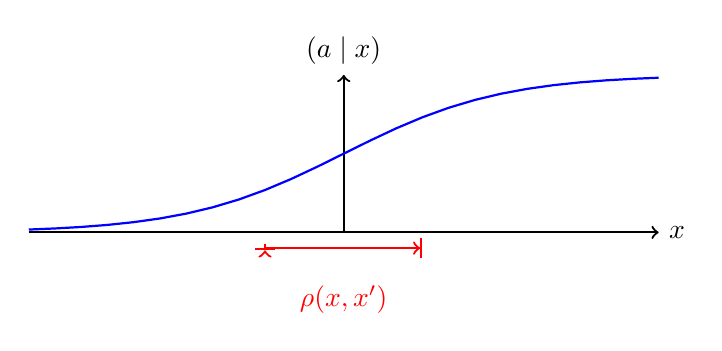
\begin{tikzpicture}[scale=2,thick,domain=-2:2]
      \draw[->] (-2,0) -- (2,0) node[right] {$x$};
      \draw[->] (0,0) -- (0,1) node[above] {$\pol(a \mid x)$};
      \draw[color=blue] plot (\x,{0.5 + 0.5 * tanh(\x)}); % node[right] {$f(x) = \frac{1}{20} \mathrm e^x$};
      \draw [|<->|,color=red] plot (-0.5,-0.1) -- node[below=1em] {$\rho(x,x')$} ++(1, 0);
    \end{tikzpicture}
    \caption{A Lipschitz function}
    \label{fig:lipschitz}
  \end{figure}
  \only<article>{
    If we wish to find the optimal policy that satisfies this constraint, then it is naturally to think about this as a constrained optimisation problem
    }
    \begin{block}{The constrained maximisation problem}
      \[
      \max_\pol \cset{\util(\pol)}{\rho(x, x')}
      \]
    \end{block}
\only<article>{
The problem in this framework is how to define the metric $\rho$ in the first place. A natural idea is to simply use the probability of $y$ as a metric. Then it doesn't matter how different $x, x'$ appear: the only important thing is how what is the distribution of $y$ implied by the different attributes. 


    \begin{block}{$\rho$ in terms of the distribution $y \mid x$}
    Firstly, assume you somehow have some probability law $\Pr$ over the variables of interest. To fix ideas, let us consider the total variation norm and assume $y \in \CY$ takes a finite number of values. Then we can define the metric as
    \begin{align}
      \rho(x, x')
      &\defn \|\Pr(y \mid x) - \Pr(y \mid x')\|_1\\
      &= \sum_{i \in \CY} \|\Pr(y \mid x) - \Pr(y \mid x')\|_1
    \end{align}
    \end{block}
  }
\end{frame}



\subsection{Bayesian fairness}
\only<article>{In both cases, we defined conditional independence for a fixed probability distribution $P_\param(x,y,z)$ on the various variables. We also considered meritocratic fairness with respect to $\param$. However, this cannot be assumed to be known. For that reason, we can assume a Bayesian approach to fairness, whereby we look at the following scores.}
\begin{frame}
  \frametitle{The Bayesian approach to fairness}
  \begin{block}{The value of a policy}
    Let $\lambda$ represent the trade-off between utility and fairness.
    \only<article>{The combined value for a given parameter $\param$ is}
    \begin{equation}
      \label{eq:combined-value}
      V(\lambda, \param, \pol) = \lambda \overbrace{U(\param, \pol)}^{\textrm{utility}} - \underbrace{(1 - \lambda) F(\param, \pol)}_{\textrm{fairness violation}}
    \end{equation}
    \only<article>{With some abuse of notation, we also define the value for a distribution $\bel$ over parameters}
    \begin{equation}
      \label{eq:combined-value}
      V(\lambda, \bel, \pol) = \int_{\Param} V(\lambda, \param, \pol) \dd \bel(\param).
    \end{equation}
  \end{block}
\end{frame}


\subsection{Further reading}

\begin{frame}
  \begin{block}{Online resources}
    \begin{itemize}
    \item COMPAS analysis by propublica \url{https://github.com/propublica/compas-analysis}
    \item Open policing database \url{https://openpolicing.stanford.edu/}
    \end{itemize}
  \end{block}
\end{frame}



%%% Local Variables:
%%% mode: latex
%%% TeX-engine: xetex
%%% TeX-master: "notes"
%%% End:
